\chapter{Grafi}
Un grafo è una generalizzazione del concetto di albero, infatti questo è un tipo speciale di grafo.
In particolare, un albero è un grafo connesso e aciclico. Questo significa che in un albero non
ci sono cicli (percorsi che iniziano e finiscono nello stesso nodo) e che tutti i nodi sono collegati
da esattamente un percorso. Se nei grafi da ogni vertice possono partire e giungere più archi,
negli alberi ogni nodo ha al massimo un padre. Un grafo viene definito come una struttura
matematica in grado di rappresentare relazioni tra oggetti.
E composto da un insieme di nodi
(o vertici) e un insieme di archi che collegano coppie di nodi. I nodi rappresentano entit`a,
mentre gli archi rappresentano le relazioni tra di esse.
\subsection{Definzioni sui Grafi}
\begin{definition}
    Un grafo \textbf{$G=(V,E)$} è costituito da un insisme di vertivi $V$ ed un insieme di archi $E$ ciascuno dei quali connette due vertici $V$ detti estremi dell'arco.\\
\end{definition}
\begin{definition}
Un grafo è \textbf{orientato} quando esiste una relazione d’ordine tra gli estremi degli
archi, ovvero gli archi hanno un verso e una direzione definita, espressi tramite una freccia.
Immaginiamo un arco come una freccia che va dalla coda alla testa, infatti il primo estremo si
dice coda ed il secondo testa\\
\end{definition}
\begin{definition}
    Un grafo si dice \textbf{denso} se il numero di archi presenti è molto vicino al numero totale di possibili archi\\
\end{definition}
\begin{definition}
    Un \textbf{cappio} è un arco i cui estremi coincidono\\
\end{definition}
\begin{definition}
Un grafo orientato è \textbf{semplice} se non ci sono cappi e non ci sono due archi con gli
stessi estremi. Se esistessero due archi con gli stessi estremi si definirebbe \textbf{multigrafo}.\\
\end{definition}
\begin{definition}
Se un grafo è semplice possiamo identificare un arco con la coppia dei suoi estremi:
$e= uv \in E$, in questo caso diciamo che l’arco $e$ è \texttt{incidente} in $u$ e in $v$.
Se il grafo è orientato, la coppia $uv$ è ordinata. In questo caso diciamo che l’arco $e$ \texttt{esce} da
$u$ ed \texttt{entra} in $v$.
Se $e = uv \in E$ diciamo che il vertice $v$ è \texttt{adiacente} al vertice $u$. Se il grafo non è orientato
la relazione di adiacenza è simmetrica\\
\end{definition}
\begin{definition}
    Il \textbf{grado $\delta(v)$} del vertice $v$ è il numero di archi incidenti in $v$\\
    Se il grafo è orientato abbiamo:
    \begin{itemize}
        \item grado entrante $\delta^-(v)$ che rappresenta il numero di archi entranti in $v$
        \item grado uscente $\delta^+(v)$ che rappresenta il numero di archi uscenti in $v$
    \end{itemize}
    \noindent Un nodo \textbf{pozzo} è un nodo che ha grado uscente pari a zero, $\delta^+(v)=0$.\\
\end{definition}
\begin{definition}
Un \textbf{percorso} $\pi$ di lunghezza $k$ dal vertice $u$ al vertice $v$ in un grafo $G = (V, E)$ è
una sequenza di $k+1$ vertici $\pi= x_0, x_1, x_2,···, x_k$ tali che $x_0 = u, x_k = v$ e $x_{i-1}x_i \in E$ per $i
= 1, . . . , k$.
Il percorso $\pi = x_0$ ha lunghezza $k = 0$.
Se $k>0$ e $x_0 = x_k$ diciamo che il percorso è \textbf{chiuso}\\
\end{definition}
\begin{definition}
Un cammino è un percorso i cui vertici $x_0, x_1,···, x_k$ sono tutti diversi con la
possibile eccezione di $x_0 = x_k$, nel qual caso esso è un \textbf{ciclo}.\\
Un ciclo di lunghezza $k=1$ è un \textbf{cappio}\\
Un \textbf{grafo aciclico} è un grafo che non contiene cicli\\
Quando esiste almeno un cammino dal vertice $u$ al vertice $v$ diciamo che il vertice v è
\textbf{accessibile} o raggiungibile da $u$.\\
\end{definition}
\begin{definition}
Un grafo non orientato si dice \textbf{connesso} se esiste almeno un cammino tra ogni
coppia di vertici.\\
Le componenti connesse di un grafo sono le classi di equivalenza dei suoi vertici rispetto
alla relazione di accessibilità. Quando si parla di componente connessa di un grafo, si fa
riferimento ad un gruppo di nodi del grafo in cui esiste un percorso da qualsiasi nodo del gruppo
verso qualsiasi altro nodo del gruppo. La ”relazione di accessibilità” a cui si fa riferimento è
semplicemente la possibilità di raggiungere un nodo da un altro attraverso uno o più archi nel
grafo. Le ”classi di equivalenza” a cui si fa riferimento sono insiemi di nodi che sono considerati
equivalenti in termini di accessibilità. Dunque, due nodi appartengono alla stessa classe di
equivalenza se e solo se sono raggiungibili tra loro attraverso archi nel grafo. Nei grafi orientati
la proprietà di raggiungibilità non è simmetrica, quindi va verificata in entrambi gli estremi del
cammino.\\
\end{definition}
\begin{definition}
    Un grafo orientato si dice \textbf{fortemente connesso} se esiste almeno un cammino da ogni vertice $u$ ad ogni altro vertice $v$.\\
\end{definition}
\begin{definition}
    Un \textbf{sottografo} del grafo $G = (V, E)$ è un grafo $G’ = (V’, E’)$ tale che $V' \subseteq V$ e
$E' \subseteq E$.
Il sottografo di $G = (V, E)$ indotto da $V' \subseteq V$ è il grafo $G’ = (V’, E’)$ tale che $E'
= {uv : uv \in 
E \text{ e } u,v \in V'}$\\.
\end{definition}
\section{Rappresentazione di un grafo}
Ci sono due modi per rappresentare un grafo $G= (V, E)$: con le liste di adiacenza oppure con
la matrice di adiacenza. La rappresentazione di tale grafo mediante le liste delle adiacenza
utilizza liste $Adj[u]$ con $u \in V$, in cui vengono memorizzati i vertici adiacenti al vertice $u$.\\
\begin{figure}[H]
    \centering  
    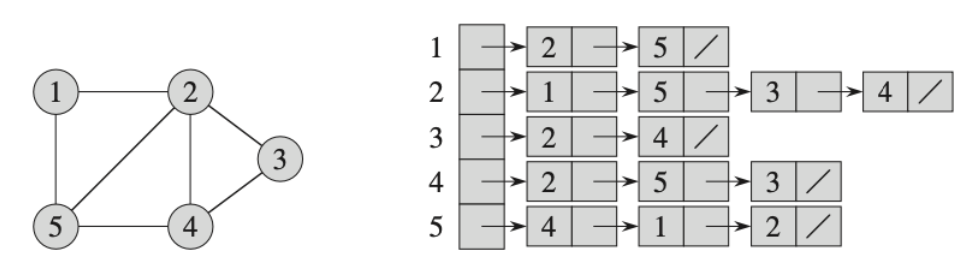
\includegraphics[width=0.5\linewidth]{../images/rappresentazione_grafo.png}
    \caption{caption}
    %\label{label}
\end{figure}
\noindent Nella rappresentazione di $G= (V, E)$ mediante la matrice di adiacenza assumiamo che i vertici
siano numerati da $1$ fino a $|V|$, la rappresentazione è costituita da una matrice booleana $A$ tale
che:\\
$
\begin{cases}
1 \text{ se } ij \in E\\
0 \text{ se } ij \notin E   
\end{cases}
$\medskip\\
\noindent Esempio con il grafo precedente:\\
\begin{figure}[H]
    \centering  
    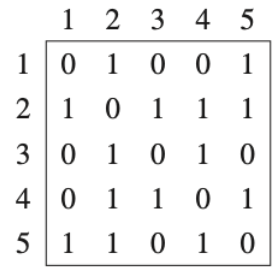
\includegraphics[width=0.25\linewidth]{../images/esempio_grafo.png}
    \caption{caption}
    %\label{label}
\end{figure}
\noindent Una matrice di adiacenza di un grafo non orientato è sempre simmetrica. Per quanto
concerne l’efficienza di queste due rappresentazioni, bisogna considerare che la lista di adiacenza
richiede spazio in memoria pari a $|V|+ |E|$, dove $|V|$ indica la cardinalità di $V$ (il numero di
vertici $=$ il numero di puntatori alle liste collegate), mentre $|E|$ indica il numero degli elementi
delle liste. La rappresentazione mediante matrice di adiacenza invece richiede spazio per una
matrice di dimensione $|V|^2$ questo significa che se un grafo è denso converrà utilizzare la matrice
delle adiacenze.
\section{Visita in ampiezza BFS}
Dato un grafo $G = (V, E)$ e un vertice distinto $s$, detto sorgente la visita in ampiezza BFS
(breadth-first search) ispeziona gli archi di $G$ per visitare tutti i vertici che sono raggiungibili
da $s$.\\
\begin{figure}[H]
    \centering  
    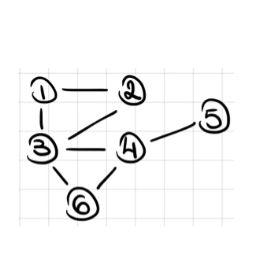
\includegraphics[width=0.25\linewidth]{../images/bfs.png}
    \caption{caption}
    %\label{label}
\end{figure}
\noindent Si parte dal nodo sorgente, la cui scelta è arbitraria, per poi
propagarsi in ampiezza; dunque, preso $1$ gli attribuisco la distanza 
da sè stesso, ovvero zero. Al secondo passo allargo l’area
fino ad includere i nodi $2$ e $3$, che inserisco in una coda ed 
incremento di uno la distanza dalla sorgente. Dopodichè espando
l’area ai vicini di questi ultimi nodi visitati, così via fino a visitare tutto il grafo.\\
Produce l'albero di visita in ambiezza i cui rami sono cammini di lunghezza minima.\bigskip\\
Si espande uniformemente la frontiera tra i vertici scoperti e quelli non ancora scoeprti, 
in altre parole, scopre tutti i vertici a distanza $k$ da $s$ prima di scoprire quelli a distanza $k+1$\\
Per mantenere traccia del punto a cui si è arrivati nell'esecuzione dell'algoritmo, i vertici sono colorati:
\begin{itemize}
    \item bianco (vertici non ancora raggiunti)
    \item grigio (vertici raggiunti che stanno sulla frontiera)
    \item nero (vertici raggiunti che non stanno sulla frontiera)
\end{itemize}
\begin{figure}[H]
    \centering  
    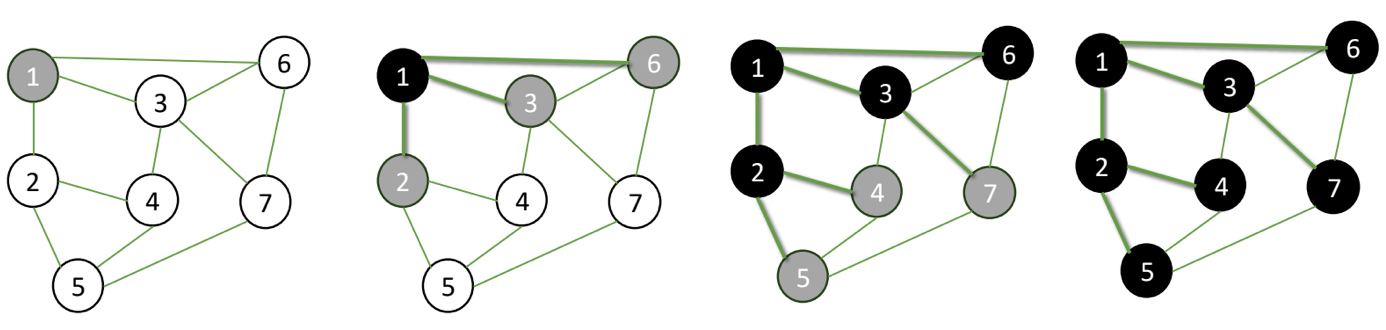
\includegraphics[width=0.5\linewidth]{../images/percorso_bfs.png}
    \caption{caption}
    %\label{label}
\end{figure}
\subsection{Pseudocodice BFS}
\begin{verbatim}
1   BFS (G, S)  // S = sorgente, G = grafo
2   foreach u in G.V = {S} // per ogni nodo appartenente al grafo, escludendo la sorgente
3       u.color = ”BIANCO”
4       u.d = infinity
5       u.p = nil
6   end     
7   s. color = ”GRIGIO”
8   s.d = 0
9   s.p = nil // il padre della sorgente non e’ nessuno
10  Q = 0
11  ENQUEUE (Q, S) // inserisco nella coda la sorgente
12  while Q != 0
13      u = DEQUEUE (Q) // visito il nodo u e lo tolgo dalla frontiera
14      foreach v in G.adj[u] // scansiono la lista delle adiacenze del vertice u
15          if v.color = ”BIANCO”
16              v.color = ”GRIGIO” // aggiungo alla frontiera ogni vertice v della lista di u
17              v.d = u.d +1
18              v.p = u
19              ENQUEUE (Q, v) // metto v in coda
20          end
21      end
22      u.color = ”NERO”
23  end
\end{verbatim}
\subsection{Analisi}
La visita viene detta in ampiezza perchè l’algoritmo espande uniformemente la frontiera; infatti,
scopre tutti i vertici a distanza $k$ dalla sorgente $s$ prima di scoprire quelli a distanza $k+1$. Per
mantenere traccia dell’esecuzione dell’algoritmo i vertici vengono colorati di bianco (vertici
non raggiunti), grigio (vertici raggiunti nella frontiera) e nero (vertici raggiunti che non sono
nella frontiera). Inizialmente l’algoritmo effettua un ciclo preliminare su ogni vertice esclusa la
sorgente del grafo, modificandone il colore in ”BIANCO”, ponendo la distanza di ogni vertice
dalla sorgente ad infinity e assegnando come predecessore null. Dopodichè vengono modificati
i campi della sorgente, ponendo il colore a ”GRIGIO” in quanto dobbiamo visitarlo e quindi
inserendolo nella frontiera e ponendo la sua distanza dalla sorgente pari a 0 ed infine aggiungo il
vertice sorgente alla coda, perchè, come detto, è stato aggiunto alla frontiera. In seguito, viene
svolto un ciclo while sulla coda $Q$ dove si itera su ogni nodo. Inizialmente viene richiamata la
funzione $DEQUEUE$ che restituisce il nodo appena rimosso dalla coda, questo sta a significare
che sto visitando il nodo appena rimosso. Dopodichè effettuo un ciclo su tutti i nodi della lista
delle adiacenze del nodo $u$ (ovvero tutti i nodi che sono collegati al nodo u) aggiungendoli in
lista solo se essi sono colorati di ”BIANCO” ovvero che non sono presenti in coda e quindi nella
frontiera, incrementando la loro distanza dalla sorgente e ponendo il loro colore a ”GRIGIO”
in quanto li inserisco nella frontiera. Procedendo con questo ragionamento si vanno a visitare
per ampiezza tutti i vertici del grafo. La complessità dell’algoritmo BFS è $O(|V|+ |E|)$, dove
$|V|$ è il numero di vertici del grafo e $|E|$ è il numero di archi del grafo.\bigskip\\
\noindent Per dimostrare la correttezza di BFS ci occorre prima dimostrare $3$ proprietà intermedie dell'algoritmo:
\begin{itemize}
    \item proprietà delle distanze
    \item proprietà del limite superiore
    \item proprietà della coda
\end{itemize} 
\subsection{Proprietà delle distanze}
Sia $G = (V, E)$, un grafo e $s \in V$ un vertice arbitrario. Allora per ogni arco $(u,v) \in E$ si ha
che:\\
$$d(s,v) \le d(s,u) + 1$$\\
\begin{proof}
\leavevmode\\
Per dimostrare questa proprietà dobbiamo considerare due casi:
\begin{enumerate}
    \item $u$ non è raggiungibile da $s$
    \item $u$ è raggiungibile da $s$
\end{enumerate}
\noindent \textbf{Caso 1}\\
E’ noto come nell’algoritmo BFS vengono inizializzate ad $\infty$ le distanze di tutti i nodi dalla
sorgente. Se $u$ non è raggiungibile da $s$, significa che non verrà mai aggiunto alla coda e la sua
distanza $u.d$ da $s$ rimarrà $\infty$. Se $u$ non è raggiungibile da $s$, non lo è neanche v allora $v.d =
\infty$, che verifica la diseguaglianza.\\
\textbf{CAso 2}\\
Se $u$ è raggiungibile da $s$, significa che $u.d$ viene aggiornato con la distanza da $u$ ad $s$ che 
chiameremo $d(s, u)$, se questo cammino passa già per $v$, allora banalmente è verificata $d(s,v) < d(s,u)$,
se invece il cammino non passa per $v$, allora aggiungendo l’arco $(u, v)$ si ha che $d(s,v) = d(s,u) + 1$,
da cui segue la diseguaglianza
\end{proof}
\subsection{Proprietà del limite superiore}
Sia $G = (V, E)$ un grafo e supponiamo che BFS venga eseguita da un nodo $s \in V$ arbitrario
(sorgente). Allora per ogni vertice $v \in V$, la distanza $v.d$ calcolata da BFS è sempre tale che:\\
$$v.d \ge d(s,v)$$\\
\begin{proof}
    \leavevmode\\
    Per dimostrare questa proprietà dobbiamo farlo per induzione\\
    \textbf{Passo base:}\\
    Il passo base è rappresentato dall’inizializzazione della BFS nella quale tutte le distanze dei
    vertici del grafo dalla sorgente sono poste ad $\infty$, quindi si ha banalmente che per ogni nodo $u$
    diverso da $s$:\\
    $$u.d= \infty \ge d(s,u)$$\\
    Per quanto riguarda la sorgente viene posta $s.d= 0$ che banalmente è uguale a $d(s, s)$. Quindi
    possiamo concludere dicendo che il passo base verifica la proprietà del limite superiore.\\
    \textbf{Passo induttivo:}\\
    Supponiamo che la diseguaglianza $u.d \ge d(s,u)$ sia vera fino a prima della riga
    $$v.d= u.d + 1$$
    dopo essere stata eseguita per ipotesi induttiva sappiamo che $u.d + 1 \ge d(s,u) + 1$, dalla proprietà 
    delle distanze abbiamo che $d(s,u) + 1 \ge d(s,v)$, allora mettendo insieme tutte le disuguaglianze 
    si ha: $v.d= u.d + 1 \ge d(s,u) + 1 \ge d(s,v)$, ottenendo così $v.d \ge d(s,v)$.
\end{proof}
\subsection{Proprietà della coda}
Si considera l’esecuzione di BFS su un grafo $G = (V, E)$ e supponiamo che la coda $Q$ contenga
i vertici $<v_1,v_2,...,v_r >$ (con $v_1$ inizio e $v_r$ fine della coda), allora si ha che:
\begin{enumerate}
    \item $v_r .d \le v_1 .d+ 1$ 
    \item $v_i .d \le v_{i+1}.d \text{ per ogni }i \text{ in } 1,2,...,r-1$
\end{enumerate}
\begin{proof}
    \leavevmode\\
Per dimostrare questa propriteà dobbiamo farlo per induzione\\
\textbf{Passo base:}\\
Dopo l’inizializzazione la coda contiene solo $s$, allora la proprietà è verificata.\\
\textbf{Passo induttivo:}\\
\textbf{1.} Assumiamo che sia vera la seguente disuguaglianza:\\
$$v_r .d \le v_1 .d+ 1 \le v_2 .d+ 1$$
Quando $v_1$, viene estratto dalla coda, $v_2$ diventa la nuova testa e si ha banalmente\\
$$v_r .d \le v_2 .d+ 1$$
\textbf{2}. Sia $v_r$ l’ultimo elemento in coda, prima di essere stato inserito in coda è stato posto
$v.d= u.d + 1$, con $u$ il primo elemento della coda ovvero $v_1$, quindi $v_r .d= v_1 .d + 1$. 
Ipotizziamo venga aggiunto un altro vertice tale per cui l’ultimo elemento è $v_{r+1}$. Si ha che
$v_{r+1} .d= v_1 .d + 1$. Per ipotesi induttiva, inoltre, si ha che $v_r .d \le v_1 .d + 1$ ma allora:
$v_r .d \le v_1 .d+ 1 = v_{r+1} .d$\\
da cui:\\
$$v_r .d \le v_{r+1} .d$$
\end{proof}
\subsection{Correttezza della BFS}
L’algoritmo BFS visita tutti i vertici raggiungibili da $s$ e quando termina $v.d = d(s, v)$ per
ogni vertice $v$ del grafo. Inoltre per ogni vertice $v \neq s$ raggiungibile da s:
\begin{itemize}
    \item $u=v.p \neq nil$
    \item $(u,v) \in E$
    \item $d(s,v) = d(s,u)+1$
\end{itemize}
\begin{proof}
    \leavevmode\\
Se $v$ non è raggiungibile da $s$ allora dalla proprietà del limite superiore si ha che\\
$$v.d=d(s,v)=\infty$$\\
Questo valore rimarrà invariato per tutta l’esecuzione dell’algoritmo, questo significa che il
vertice $v$ non verrà mai aggiunto in coda e quindi i vertici non raggiungibili non vengono visitati
da BFS.\\
Se $v$ è raggiungibile da $s$, per ogni vertice $v \in V$ raggiungibile da $s$ i seguenti punti vengono
effettuati una ed una sola volta:
\begin{enumerate}
    \item a $v.color$ viene assegnato il colore "GRIGIO"
    \item a $v.d$ viene assegnato il valore $d(v,s)$
    \item se $v$ è diverso da $s$, a $v.p$ viene assegnato un vertice $u$ tale che $d(s,v)=d(s,u)+1$, se $v=s$ a $s.p$ è assegnato nil
    \item il vertice $v$ viene aggiunto alla coda $Q$
\end{enumerate}
\noindent Dopo l'inizializzazione nessun vertice viene più colorato di $BIANCO$, 
un vertice può essere colorato di $GRIGIO$ soltanto se era $BIANCO$\\ 
Se consideriamo la sorgente banalmente l'inizializzazione avviene una sola volta quindi:
\begin{itemize}
    \item $s.color="GRIGIO"$
    \item $s.d=0$
    \item $s.p=nil$
    \item $ENQUEUE(Q, S)$
\end{itemize}
\noindent Si considera poi un insieme di vertici\\
$$V_k={v \in V : d(s,v)=k}$$\\
ovvero l’insieme di vertici posti a distanza $k$ da $s$. Sia $v \in V_k$, durante l’esecuzione del ciclo
while la coda $Q$ non è mai vuota e non appena il vertice $v$ viene messo in coda i valori $v.d$ e
$v.p$ non possono più cambiare in quanto a $v.color$ viene assegnato il colore ”GRIGIO” e per
entrare nell’if è richiesto che $v.color$ sia ”BIANCO”, di conseguenza se l’ordine di inserimento
in coda è\\
$${s=v_0, v_1,...,v_t}$$\\
banalmente si ha che\\
$$v_i .d \le v_{i+1} .d$$\\
che corrisponde alla proprietà della coda. Il vertice $v$ a distanza $k$ non può essere scoperto
prima, in quanto non è adiacente a nessun vertice a distanza minore $k-1$, infatti a tale distanza
è presente $u$ distante da $s$ $k-1$, a cui $s$ è adiacente.
\end{proof}
\newpage
\section{DFS}
L’algoritmo DFS (deep-first search) visita in profondità un grafo, ispezionando gli archi uscenti
a partire dall’ultimo vertice $v$ scoperto. Quando tutti gli archi di $v$ sono stati ispezionati ”torna
indietro” per ispezionare i restanti archi del vertice da cui $v$ era stato scoperto
\subsection{Pseudocodice}
\begin{verbatim}
    DFS(G,s){
        foreach u in G.V
            u.color = "BIANCO"
            u.p = nil
            time = 0
        foreach u in G.v
            if u.color = "BIANCO"
                DFS_VISIT(G, u)
    }
    DFS_VISIT{
        time = time + 1
        u.d = time // istante di scoperta
        u.color = "GRIGIO"
        foreach v in G.adj[u]
            if v.color = "BIANCO"
                v.p = u
                DFS_VISIT(G, v) // chiamo ricorsivamente sul primo sul primo nodo non ancora scoperto
        time = time + 1
        u.f = time // istante di completamento
        u.color = "NERO"
    }
\end{verbatim}

\begin{figure}[H]
    \centering  
    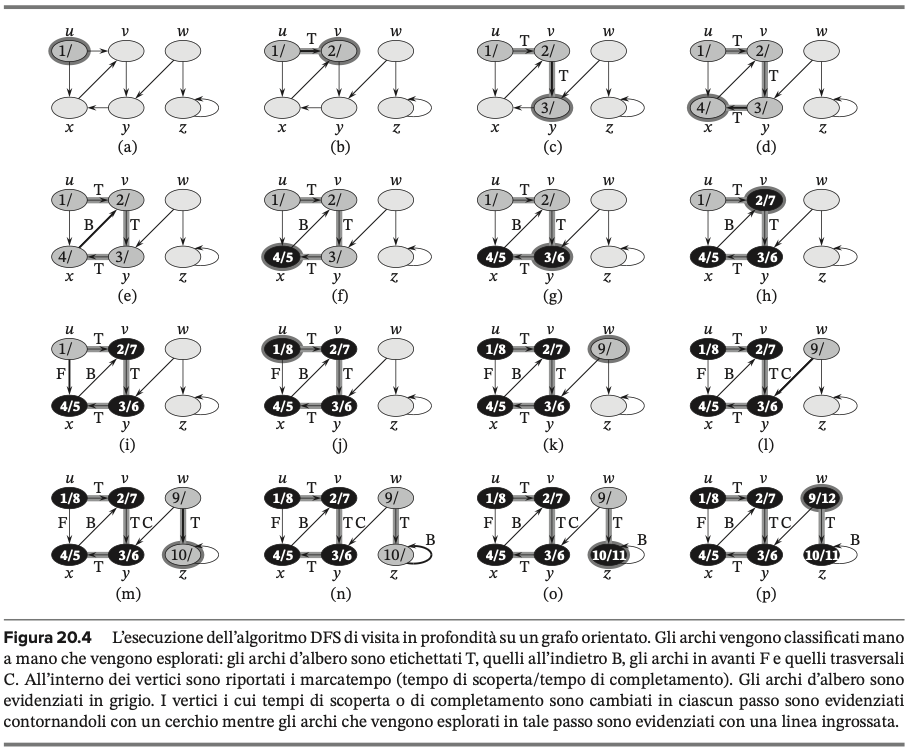
\includegraphics[width=0.90\linewidth]{../images/dfs.png}
\end{figure}

\subsection{Analisi}
DFS pone due marcatempi su ogni vertice $u$, in particolare il primo identifica il tempo di scoperta 
$(u.d)$ e viene assegnato quando $u$ diventa \textbf{grigio}, mentre il secondo marcatempo identifica
il tempo di completamento $(u.f)$ ossia quando il vertice è completato e colorato di \textbf{nero}. DFS
inizializza il colore di tutti i vertici a \textbf{bianco} e inizializza una variabile globale che identifica il
tempo. Successivamente chiama \textbf{DFS\_VISIT} sui vertici $u$ che non sono stati ancora visitati.
All’interno di DFS\_VISIT viene incrementata la variabile tempo e viene assegnato al primo
marcatore di $u$, indicandone l’istante in cui viene colorato di $"GRIGIO"$. Dopodichè si prende
la lista di adiacenza del nodo $u$ e si scorre richiamando \textbf{ricorsivamente} DFS\_VISIT sul nodo $v$
facente parte della lista di $u$. Infine viene incrementata nuovamente la variabile tempo e viene
assegnata al marcatore di completamento di $u$. La complessità di DFS è \textbf{$O(|V|+ |E|)$}, dove
\textbf{$|V|$} è il numero di vertici del grafo e \textbf{$|E|$} è il numero di archi del grafo.
\subsection{Proprietà delle parentesi}
Se si rappresenta:
\begin{itemize}
    \item la scoperta di ogni vertice $u$ con una parentesi aperta $(_u$ e 
    \item il completamento con una parentesi chiusa $_u)$
\end{itemize}
\noindent si ottiene una sequenza bilanciata di parentesi.\\
Ossia, per ogni coppia di vertici $u$ e $v$, ci sono quattro possibilità:
\begin{enumerate}
    \item $(_u ... _u)...(_v ... _v)$
    \item $(_v ... _v)...(_u ... _u)$
    \item $(_u ...(_v ... _v)... _u)$
    \item $(_v ...(_u ... _u)... _v)$
\end{enumerate}
\begin{figure}[H]
    \centering  
    \includegraphics[width=1\linewidth]{../images/proprietà parentesi.png}
\end{figure}
\subsection{Teorema delle Parentesi}
\colorbox{SALZO}{\parbox{\dimexpr\linewidth-2\fboxsep}{\begin{theorem}
In una qualsiasi DFS di un grafo $G = (V, E)$ (orientato o non orientato), per ogni coppia di
nodi $u, v$ è soddisfatta una e una sola delle seguenti tre condizioni:
\begin{enumerate}
    \item Gli intervalli $[u.d, u.f]$ e $[v.d, v.f]$ sono completamente disgiunti; $u$ e $v$ non sono discendenti
uno dell’altro nella foresta della visita in profondità
    \item L’intervallo $[u.d, u.f]$ è interamente contenuto nell’intervallo $[v.d, v.f]$ e $u$ è un discendente
di $v$ in un albero di visita in profondità
    \item L’intervallo $[v.d, v.f]$ è interamente contenuto nell’intervallo $[u.d, u.f]$ e $v$ è un discendente
di $u$ in un albero di visita in profondità. 
\end{enumerate}   
\end{theorem}}}
\begin{proof}
    \textbf{Caso $u.f < v.d$}\\
    Sapendo che $u.d < u.f < v.f$ ne segue che:\\
    $$ u.d < u.f < v.d < v.f $$\\
    e si decide che i due intervalli non hanno intersezione e quindi sono disgiunti. Bisogna notare che essendo 
    i due intervalli disgiunti si ha che il vertice $v$ viene scoperto dopo che il nodo $u$ è stato visitato, 
    segue che non esiste un cammino che congiunge $u$ e $v$.\\
    \textbf{Caso $u.f > v.d$}\\
    In questo caso si ha che il vertice $v$ viene scoperto quando $u$ è grigio (in esplorazione), quindi
    la lista delle adiacenze di $v$ viene completamente esplorata prima di riprendere l’esplorazione
    di $u$ e pertanto $v$ viene completato prima di $u$.
\end{proof}
\subsection{Teorema del cammino bianco}
\colorbox{SALZO}{\parbox{\dimexpr\linewidth-2\fboxsep}{\begin{theorem}
In una foresta di visita in profondità di un grafo $G = (V, E)$ (orientato o non orientato), il
vertice $v$ è discendente del vertice $u$ se e solo se, al tempo $u.d$ quando $u$ viene scoperto il vertice
$v$ può essere raggiunto da $u$ lungo un cammino che è formato esclusivamente da vertici bianchi.
\end{theorem}}}
\begin{proof}
    $\Rightarrow )$ Sia $v$ un discendente di $u$, sia $P=x_0, x_1,....,x_k$ (con $x_0=u$ e $x_k=v$) la sequenza 
    dei vertici da $u$ a $v$. Sapendo che $x_{i+1}$ viene scoperto dalla lista delle adiacenze di $x_i$, esiste 
    l'arco ($x_i, x_{i+1}$) e banalmente $x_i$ viene visitato prima di $x_{i+1}$. Quindi nel cammino P quando 
    $x_0 = u$ viene scoperto, tutti i nodi sucessivi ancora non sono stati scoeprti e quindi sono bianchi.\\
    $\Leftarrow )$ Supponiamo che quando u viene scoperto esista un cammino bianco da $u$ a $v$, allora essendo
    che $v$ viene scoperto dopo $u$, dalla proprietà delle parentesi si ha che\\
    $$(u...u)...(v...v)$$\\
    quindi sono disgiunti, oppure\\
    $$ (u...(v...v)...u)$$\\
    quindi sono discendenti.        
    Supponiamo per assurdo che\\
    $$(u...u)...(v...v)$$
    e che quindi $v$ non sia discendete di $u$. Si può assumere che $v$ sia il primo vertice del cammino
    bianco che non è discendete di $u$. Sia $w = x_{k-1}$, il vertice che precede $v$ nel cammino bianco.
    Siccome $w$ è discendente di $u$ per la proprietà delle parentesi si ha che\\
    $$(u...(w...w)...u)...(v...v)$$\\
    ma questo è assurdo in quanto $v$ è nella lista delle adiacenze di $w$ e quindi deve essere scoperto
    prima che $w$ sia completato. Quindi si conclude che $v$ è discendete di $u$.    
\end{proof}
\subsection{Tipi di archi DFS}
Sia $uv \in E$ un arco, questo può essere classificato in:
\begin{itemize}
    \item \textbf{Archi d'albero:} $v$ è scoperto dalle adiacenze di $u$ quindi ($v.status = UNEXPLORED$)
    \item \textbf{Archi all'indietro:} $u=v$, oppure v è ascendente di $u$ ($v.status = EXPLORING $)
    \item \textbf{Archi in avanti:} $v$ discendente di $u$ ($v.status=EXPLORED$ $AND$ $v.timestamp > u.timestamp$)
    \item \textbf{Archi trasversali:} $u$ e $v$ appartengono a rami diversi ($v.status=EXPLORED$ $AND$ $v.timestamp < u.timestamp$) 
\end{itemize}
\noindent Il timestamp a cui fanno riferimento è quello di scoperta dei nodi.\medskip\\
\colorbox{SALZO}{\parbox{\dimexpr\linewidth-2\fboxsep}{\begin{theorem}
   In una DFS di un grafo $G=(V,E)$ non orientato, gli archi di G possono essere solo archi dell'albero (T) o archi all'indietro.
\end{theorem}}}
\subsection{Ordinamento Topologico}
Un Ordinamento Topologico di un DAG (Directed Acyclic Graph) $G =(V, E)$ è un ordinamento
totale di tutti i suoi vertici tale che, se $G$ contiene un arco $(u, v)$, allora $u$ appare prima di $v$
nell’ordinamento.\medskip\\
\textbf{Topological-Sort(G)}
\begin{enumerate}
    \item Chiama DFS(G) per calcolare i tempi di completamento $v.f$ per ciascun vertice $v$
    \item Una volta completata la visita di un vertice, inserisce il vertice in testa a una lista concatenata
    \item return la lista concatenata dei vertici
\end{enumerate}
\begin{figure}[H]
    \centering  
    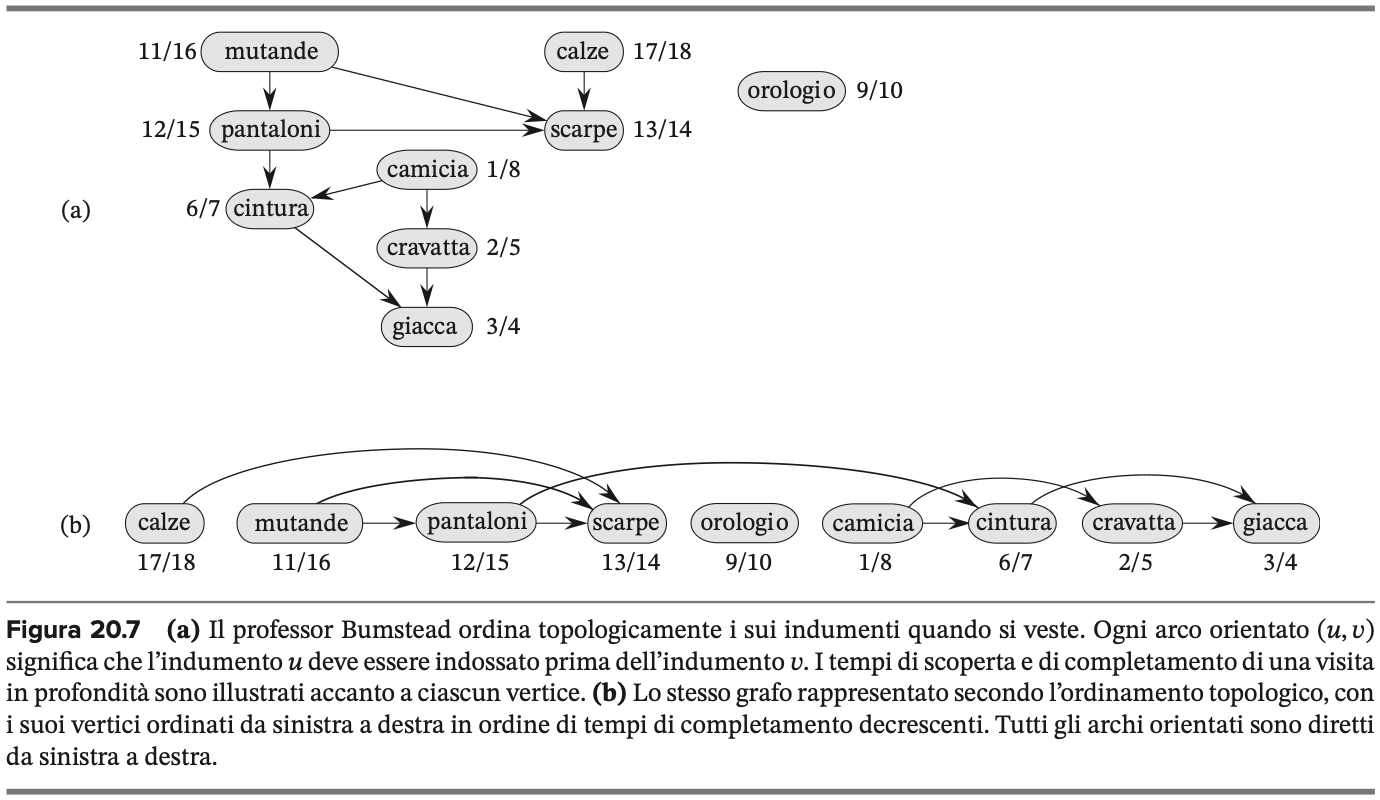
\includegraphics[width=1\linewidth]{../images/ordinamento_topologico.png}
\end{figure}
\noindent \colorbox{SALZO}{\parbox{\dimexpr\linewidth-2\fboxsep}{\begin{theorem}
   Un grafo orientato è aciclico (un DAG) se, e solo se, nella visita in profondità non si trova nessun arco all'indietro
\end{theorem}}}
\begin{proof}
    $\Rightarrow )$ Se in una visita in profondità si trova un arco all’indietro $vu$, allora tale arco aggiunto al
cammino da $u$ a $v$ (che esiste in quanto $v$ è discendente di $u$) forma un ciclo.\\
    $\Leftarrow )$ Viceversa, supponiamo che il grafo abbia un ciclo. Sia $v$ il primo vertice del ciclo ad essere
scoperto e sia $uv$ l’arco del ciclo che entra in $v$. Quando $v$ viene scoperto, esiste un cammino
bianco da $v$ ad $u$ e quindi, per la proprietà del cammino bianco, $u$ è discendente di $v$. Di
conseguenza $uv$ è un arco all’indietro.
\end{proof}
\noindent \colorbox{SALZO}{\parbox{\dimexpr\linewidth-2\fboxsep}{\begin{theorem}
   TOPOLOGICAL-SORT produce un ordinamento topologico del DAG che gli viene fornito in input
\end{theorem}}}
\begin{proof}
    Basta dimostrare che per ogni arco $uv$ il vertice $v$ viene finito prima del vertice $u$.
Quando l’arco $uv$ viene esplorato, il vertice $u$ è grigio mentre il vertice $v$ non può
essere grigio, altrimenti $uv$ sarebbe un arco all’indietro.\\
Se $v$ è nero, allora è già stato completato, mentre $u$ non lo è ancora.\\
Se $v$ è bianco, allora è discendente di $u$ per la proprietà del cammino bianco e
viene completato prima di $u$ per la proprietà delle parentesi.
\end{proof}
\subsection{Componenti fortemente connesse}
\begin{definition}
    Una componente fortemente connessa (CFC) di un grafo orientato $G = (V,E)$ è un insieme
    massimale di vertici $U \subseteq V$ tale che, $ \forall u,v \in U$ esiste un cammino da $u$ a $v$ ed un cammino
    da $v$ ad $u$.  
\end{definition}
\noindent Per trovare le componenti fortemente connesse di un grafo è sufficiente seguire questi passi:
\begin{enumerate}
    \item Chiamare DFS sul grafo e calcolare i tempi di completamento per ciascun vertice;
    \item Creare il grafo trasposto di G, ottenuto invertendo il verso di tutti gli archi;
    \item Chiamare DFS sul grafo trasposto considerando i vertici in ordine decrescente di tempo
            di completamento calcolato al punto 1.;
    \item Restituire o stampare le componenti fortemente connesse del grafo.
\end{enumerate}
\noindent \begin{figure}[H]
    \centering  
    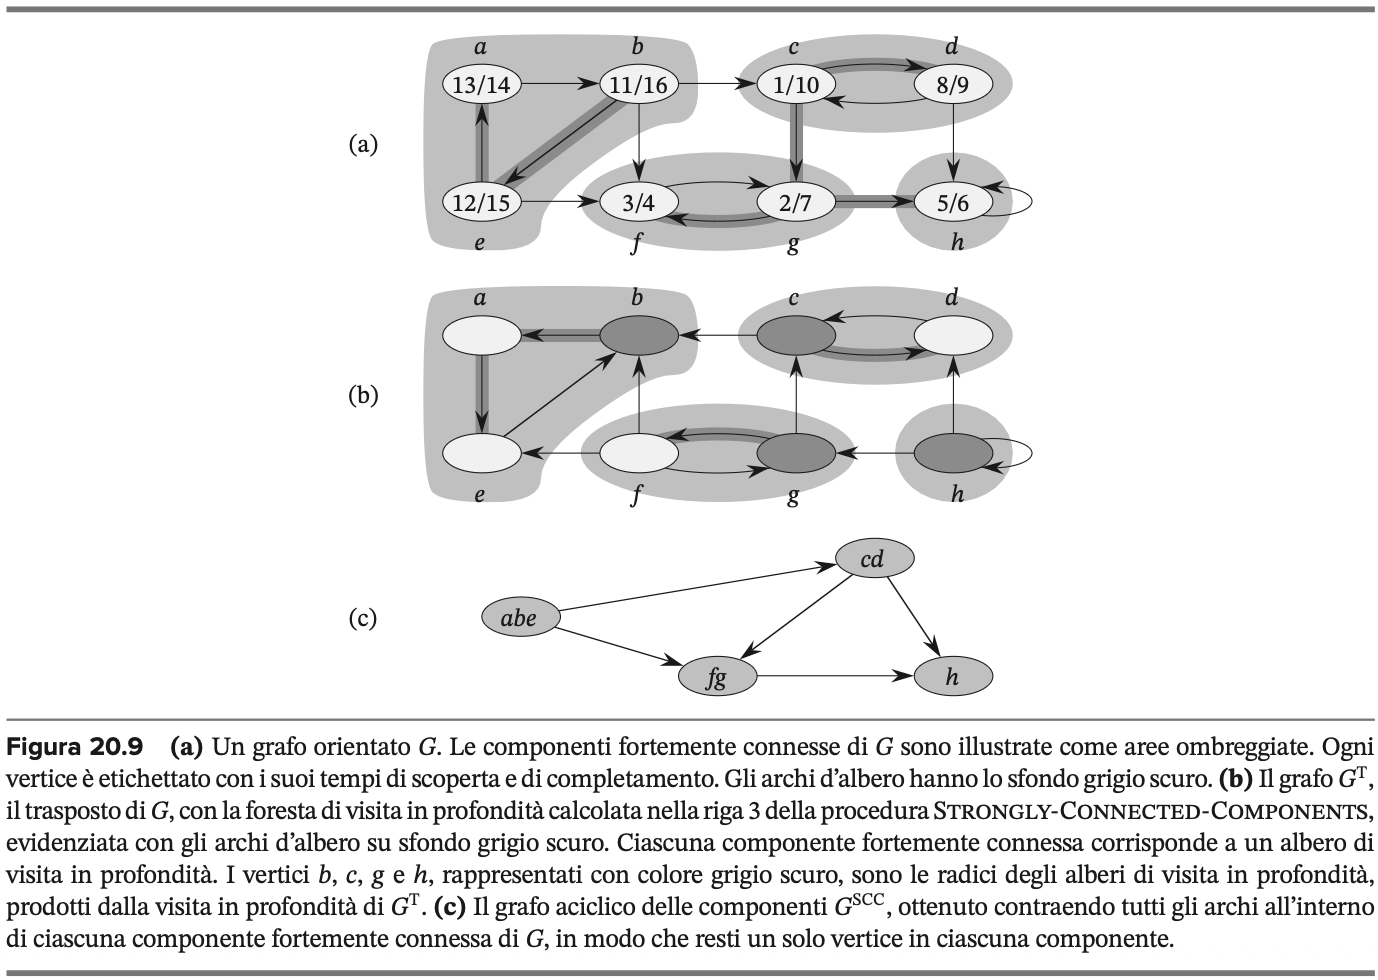
\includegraphics[width=1\linewidth]{../images/componenti fortemente connesse.png}
\end{figure}
\subsection{Grafo Trasposto $G^T$}
Dato un grafo $G=(V,E)$, il grafo trasposto $G^T=(V,E^T)$ è il grafo avente gli stessi vertici di G 
e un insieme di archi definiti come\\
$E^T=\{(u,v):(v,u) \in E\}$\\
\begin{figure}[H]
    \centering  
    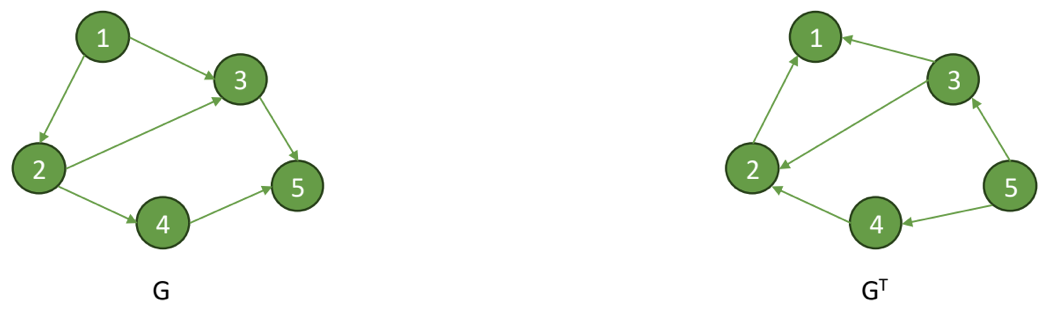
\includegraphics[width=0.80\linewidth]{../images/grafo_trasposto.png}
\end{figure}

\section{Shortest Path (Percorsi minimi)}
Il problema dei cammini minimi prende in input un grafo orientato pesato 
$G(V,E)$ con una funzione peso $\omega:E \to \mathbb{R}$ che associa ad ogni arco un numero reale 
che rappresenta il suo peso. $V$ è l'insieme dei vertici $v_1,v_2,\dots, v_n$. Il problema 
restituisce il cammino minimo (sequenza di nodi) partendo da un nodo sorgente fino ad un nodo destinazione di un grafo. Nel caso di 
grafi non pesati il cammino minimo è rappresentato dal cammino più corto, mentre nel caso di grafi pesati il cammino minimo è quello che ha peso totale minimo.\smallskip\\
Esistono numerose \textbf{varianti} ma queste sono le più importanti:
\begin{itemize}
    \item \textbf{SSPS (Single Pair Shortest Path)}: Viene fornito in input una coppia di sorgente e destinazione, e viene restituito
    il percorso minimo tra sorgente e destinazione.
    \item \textbf{SSPS (Single Source Shortest Path)}: Viene fornito in input solo la sorgente e viene restituito il percorso minimo per visitare tutti i vertici del grafo.
    \item \textbf{SDSP (Single Destination Shortest Path)}: Viene fornito in input solo la destinazione e vengono restituiti i percorsi minimi da ogni vertice del grafo.
    \item \textbf{APSP (All Pairs Shortest Path)}: Vengono restituiti tutti percorsi minimi per ogni coppia di vertici (sorgente, destinazione) del grafo. 
\end{itemize}
In generale, indichiamo il \textbf{peso di un cammino minimo} dal vertice $u$ al vertice $v$ 
con questa notazione:
\[ \omega (p) = \delta (u,v)    \]
Se un nodo \textbf{non è raggiungibile} in alcun modo allora il peso sarà:
\[  \delta (u,v) = +\infty    \]



\subsection{Proprietà}
Gli algoritmi per cammini minimi godono delle seguenti proprietà:
\begin{itemize}
    \item \textbf{Sottostruttura ottima}: ogni sotto-percorso del cammino minimo è a sua volta minimo (ottimo).
    Questa proprietà è molto importante in quanto consente l'utilizzo di algoritmi \textbf{greedy} (vd. \ref{greedy}).
    \item \textbf{Cicli}: nel caso in cui non ci sono cicli di peso negativo all'interno del grafo
    il peso del cammino minimo è ben definito. Invece nel caso in cui ci sono cicli di peso negativo
    il peso del cammino minimo non è definito e diciamo che il peso di tale cammino è $\delta(s,v) = -\infty$.
    Vediamo un esempio:
    \begin{figure}[H]
    \centering  
    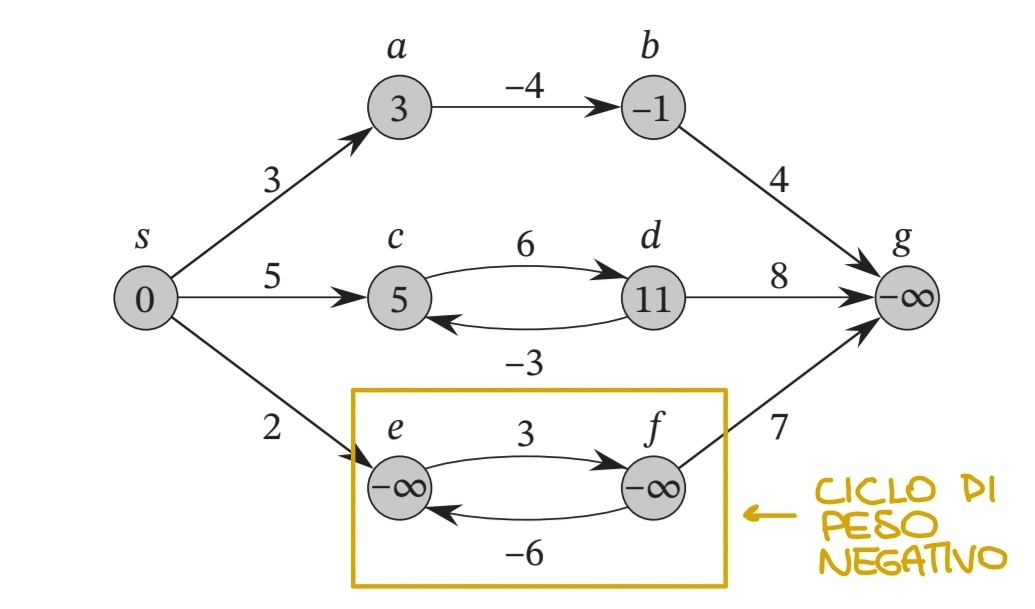
\includegraphics[width=0.70\linewidth]{../images/ciclo_negativo.jpg}
    %\label{label}
\end{figure}
    
    \item \textbf{(Non) Unicità}: I cammini minimi non sono necessariamente unici, nè lo sono gli alberi dei cammini minimi.

\end{itemize}

\subsection{Rappresentazione dei cammini minimi}
Gli algoritmi per i cammini minimi non solo calcolano il peso del cammino minimo, ma permettono di sapere 
i vertici che compongono tale cammino. Dato un grafo $G= (V,E)$ per ogni vertice $v \in V$ manteniamo 
un \textbf{predecessore} $\bm{v.\pi}$ che può essere un altro vertice o il valore \textsc{nil}. Gli algoritmi
per i cammini minimi impostano $\pi$ in modo che la catena di predecessori che inizia da un vertice $v$
percorra all'indietro un cammino minimo da $s$ a $v$. Quindi, per ogni vertice $v \neq$ \textsc{nil},
possiamo stampare un cammino minimo da $s$ a $v$.

\subsection{Rilassamento}
Gli algoritmi che vedremo usano la tecnica del \textbf{rilassamento}. Per ogni vertice $v \in V$, gli algoritmi per i cammini minimi da sorgente unica (single source) 
mantengono un attributo $v.d$ che rappresenta la \textbf{stima del cammino minimo}, ovvero il percorso provvisorio minimo che va dalla sorgente fino al vertice che stiamo analizzando.
Il processo di rilassamento di un arco $(u,v)$ consiste nel verificare se passando per $u$, è possibile migliorare il cammino minimo per $v$ precedentemente trovato.
Arrivati alla fine di questo processo quindi avremo un percorso minimo che parte da $s$ e visita tutti i vertici del grafo.\smallskip\\
Vediamo un esempio:
\begin{figure}[H]
    \centering  
    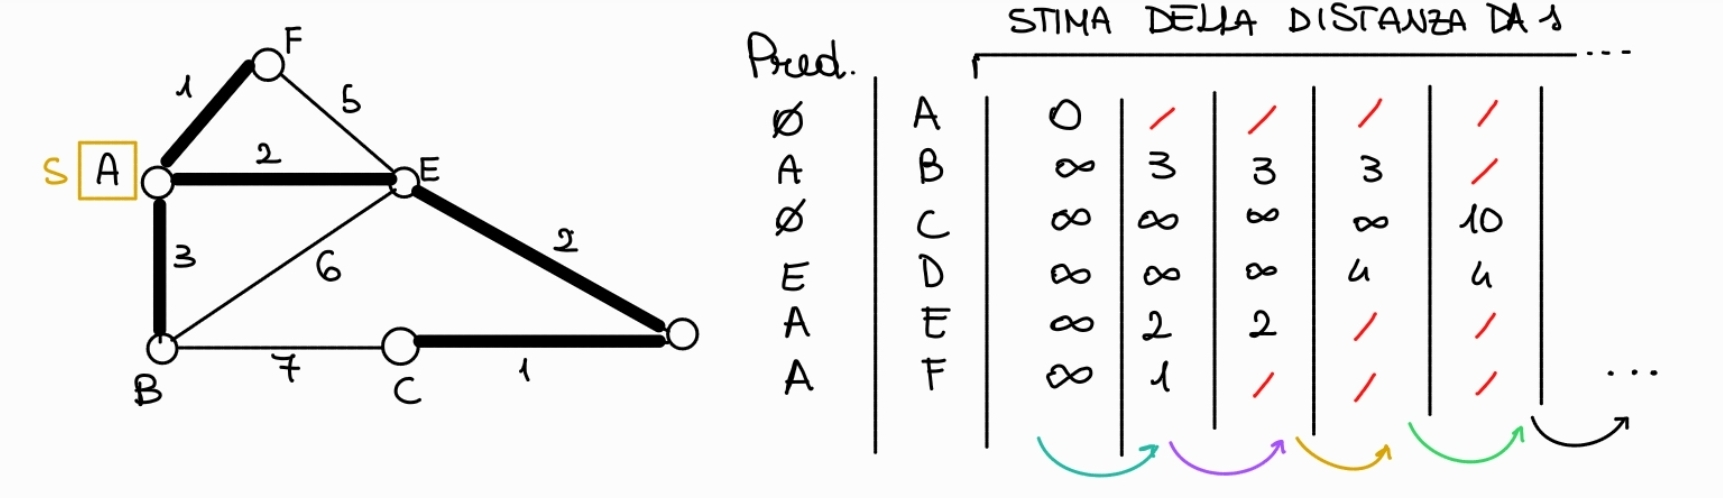
\includegraphics[width=0.9\linewidth]{../images/esempio_rilassamento}
    %\label{label}
\end{figure}
\noindent Creiamo un tabella in costante aggiornamento dove teniamo traccia dei predecessori e delle stime delle distanze. All'inizio le stime delle distanze sono impostate tutte a $\infty$
tranne la sorgente la cui distanza da se stessa è ovviamente 0. Successivamente procediamo in questa maniera:
\begin{enumerate}
    \item Seleziono la distanza stimata minima, ovvero seleziono il vertice la cui distanza stimata è minima rispetto a tutte quelle nella colonna, nel primo caso la distanza minima è 0, quindi 
    selezioniamo il vertice $A$.
    \item Una volta selezionato il vertice, verifichiamo quali vertici posso raggiungere a partire dal vertice selezionato e con che peso avviene tale raggiungimento. Nel nostro caso, abbiamo selezionato il vertice
    $A$, da $A$ possiamo arrivare a $F$ con costo 1, possiamo arrivare a $B$ con costo 3 e possiamo arrivare a $E$ con costo 2.
    \item Infine dobbiamo aggiornare la tabella con i valori che abbiamo trovato, impostando $A$ come predecessore di $A,B,E$ e aggiornando la stima delle distanze nella prossima colonna con i costi del raggiungimento di ogni vertice.
    Nella colonna successiva, quindi, ci saranno le distanze aggiornate e continueremo il processo ripartendo il con lo step (1.) (selezionando la distanza minima ecc...), mentre il nodo che avevamo in precedenza selezionato
    lo abbiamo segnato con una barra rossa. Quando aggiorniamo i dati, seguiamo il criterio principale di trovare il percorso minimo, quindi aggiorneremo un valore se e solo se è minore di quello attuale.
\end{enumerate}
Il processo di rilassamento sarà concluso quando tutta la colonna delle distanza stimate sarà composta da barre rosse, questo vorrà dire che abbiamo visitato tutti i vertici e che abbiamo delineato il cammino minimo.


\subsection{Algoritmo di Bellman-Ford}
L'algoritmo di \textbf{Bellman-Ford} risolve il problema dei cammini minimi da sorgente unica nel caso generale in cui i  pesi degli archi \textbf{possono essere negativi}.
Dato un grafo orientato pesato $G = (V,E)$ con vertice sorgente $s$ e funzione peso $w : E \rightarrow \mathbb{R}$ (ovvero che a ogni arco viene assegnato un numero reale rappresentate il suo peso), 
l'algoritmo di Bellman-Ford restituisce un valore booleano che indica se esiste un ciclo di peso negativo che
è raggiungibile dalla sorgente. Se un tale ciclo esiste, l'algoritmo indica che il problema non ha soluzione. 
Se un tale ciclo non esiste, l'algoritmo fornisce i cammini minimi e i loro pesi.
La procedura \texttt{BELLMAN-FORD} \textbf{rilassa} gli archi, riducendo progressivamente il valore stimato $v.d$ per il peso di un cammino minimo dalla sorgente $s$ a ciascun vertice $v \in V$,
fino a raggiungere il peso effettivo $\delta(s, v)$ di un cammino minimo.\smallskip\\
Ecco lo \textbf{pseudocodice}:
\begin{verbatim}
    BELLMAN-FORD(G, w, s)
    INITIALIZE-SINGLE-SOURCE(G, s)    
    for i = 1 to |G.V| - 1
        for ogni arco (u, v) in G.E
            RELAX(u, v, w)     // applica il rilassamento
    for ogni arco (u, v) in G.E
        if v.d > u.d + w(u, v)
            return FALSE
    return TRUE
\end{verbatim}
L'algoritmo restituisce \textsc{true} se e soltanto se il grafo non contiene cicli di peso negativo che sono raggiungibili dalla sorgente.\smallskip\\
Vediamo un esempio:
\begin{figure}[H]
    \centering  
    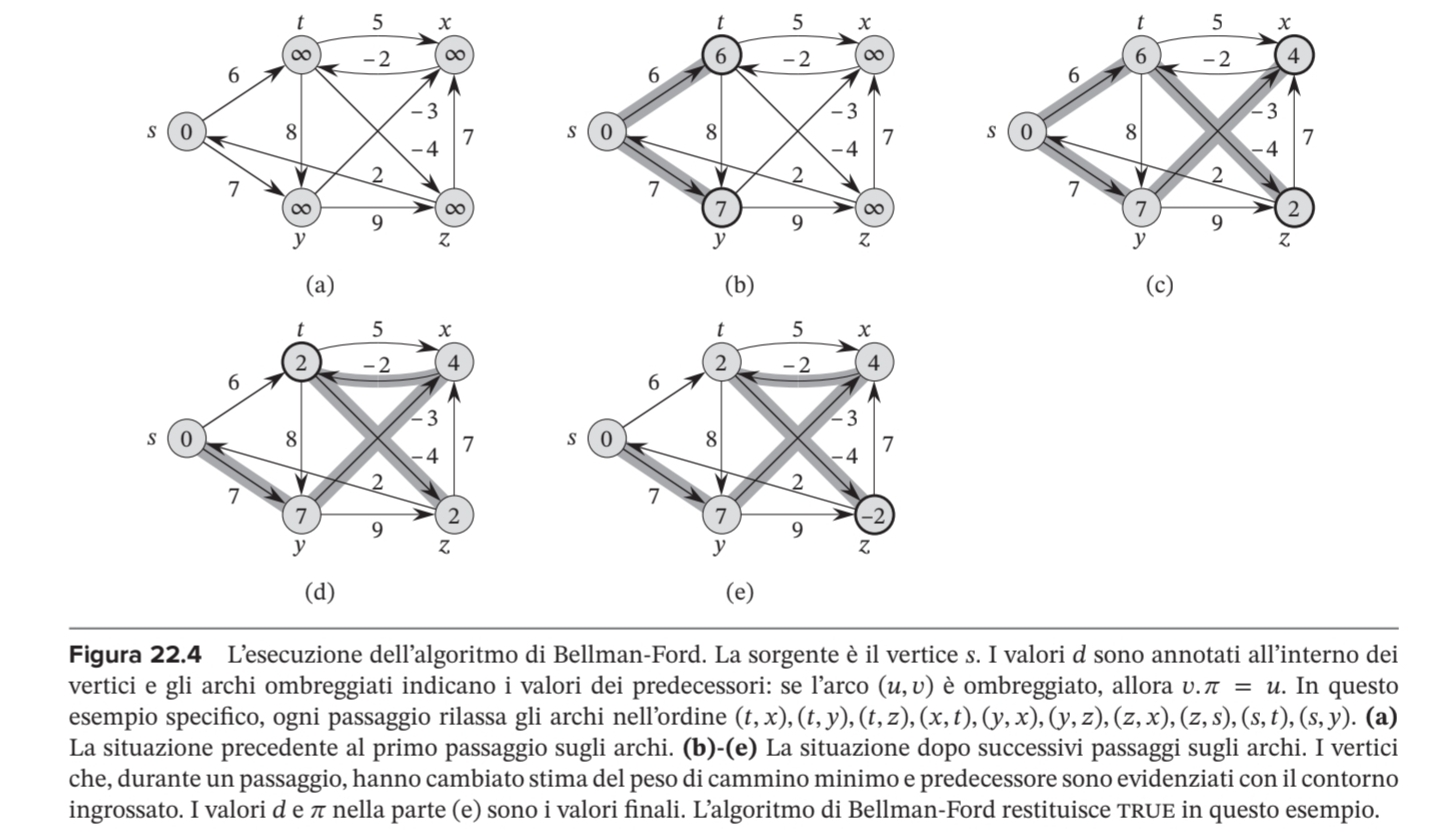
\includegraphics[width=1\linewidth]{../images/Bellman_Ford}
\end{figure}


\noindent Invece, per quanto riguarda problemi di cammino minimo da un unica sorgente con archi che \textbf{non sono mai positivi}, esiste \textbf{l'algoritmo di} \textbf{Dijkstra}, anch'esso basato sulla tecnica del rilassamento ma che non abbiamo approfondito.


\subsection{Algoritmo di Bellman Ford versione distribuita}
L'algoritmo di Bellman Ford \textbf{distribuito} si differenzia da quello che abbiamo visto in 
precedenza per queste tre caratteristiche:
\begin{enumerate}
    \item \textbf{Conoscenza locale}: ogni nodo conosce solo i per raggiungere i nodi adiacenti
    \item \textbf{Messaggistica}: i nodi si scambiano messaggi informativi contenenti i propri \textbf{distance vector},
    ovvero il vettore che contiene le distanze dagli altri nodi.
    \item \textbf{Asincronicità}: calcolo del risultato finale alla ricezione di un aggiornamento
\end{enumerate}

\noindent Questa è l'equazione con cui aggiorniamo le distanze del cammino minimo, siano $x$ e $y$ due nodi di un grafo,
l'equazione è la seguente:
\[ d_x (y) = \underset{v \in N(x)}{\min} \{ c(x, v)+ d_v (y)\}  \]
dove:
\begin{itemize}
    \item $N(x)$ è l'insieme dei vicini del nodo $x$, ovvero tutti i nodi che hanno un collegamento (arco) diretto a $x$.
    \item $v$ è un singolo nodo vicino.
    \item $y$ è il nodo di destinazione finale.
    \item $d_x(y)$ è il costo stimato da $x$ a $y$.
    \item $c(x,y)$ è il costo del link diretto verso il vicino $v$.
    \item $d_v(y)$ è la distanza da $v$ a $y$ dichiarata dal vicino. 
\end{itemize}

\noindent L'equazione con cui aggiorniamo il risultato quindi funziona così: ad ogni nodo visitato vengono analizzati 
tutti i suoi vicini, e viene scelto il cammino che minimizza la somma per arrivare a $y$.






>>>>>>> 16d05b0675fd351fa4ad45098c100dc6fb390d02
